\documentclass{article}

% if you need to pass options to natbib, use, e.g.:
%     \PassOptionsToPackage{numbers, compress}{natbib}
% before loading neurips_2019

% ready for submission
%\usepackage{neurips_2019}
\usepackage[pdftex]{graphicx}
% to compile a preprint version, e.g., for submission to arXiv, add add the
% [preprint] option:
\usepackage[preprint]{neurips_2019}

% to compile a camera-ready version, add the [final] option, e.g.:
     %\usepackage[final]{neurips_2019}

% to avoid loading the natbib package, add option nonatbib:
%     \usepackage[nonatbib]{neurips_2019}

\usepackage[utf8]{inputenc} % allow utf-8 input
\usepackage[T1]{fontenc}    % use 8-bit T1 fonts
\usepackage{hyperref}       % hyperlinks
\usepackage{url}            % simple URL typesetting
\usepackage{booktabs}       % professional-quality tables
\usepackage{amsfonts}       % blackboard math symbols
\usepackage{nicefrac}       % compact symbols for 1/2, etc.
\usepackage{microtype}      % microtypography

\title{Studying Shallow and Deep Convolutional Neural Networks as Learned Numerical
  Schemes on the 1D
  Heat Equation and Burgers' Equation}

% The \author macro works with any number of authors. There are two commands
% used to separate the names and addresses of multiple authors: \And and \AND.
%
% Using \And between authors leaves it to LaTeX to determine where to break the
% lines. Using \AND forces a line break at that point. So, if LaTeX puts 3 of 4
% authors names on the first line, and the last on the second line, try using
% \AND instead of \And before the third author name.

\author{%
  Alejandro Francisco Queiruga\\%\thank{Corresponding author} \\
  Earth and Environmental Sciences Area\\
  Lawrence Berkeley National Lab\\
  Berkeley, CA 94720\\
  \texttt{afqueiruga@lbl.gov}
}

\begin{document}

\maketitle

\begin{abstract}
  This paper examines the coincidence of neural networks with
  numerical methods for solving spatiotemporal physical
  problems. Neural networks are used to learn predictive numerical
  models from trajectory datasets from two well understood 1D
  problems: the heat equation and the inviscid
  Burgers' equation. Coincidence with established numerical methods is shown by demonstrating that a
  single layer convolutional neural network (CNN) converges to a traditional finite difference stencil for the
  heat equation. However, a discriminator-based adversarial training
  method, such as those used in generative adversarial networks (GANs), does not find the
  expected weights. A compact deep CNN is applied to nonlinear Burgers'
  equation, where the models' architecture is reminiscent of existing winding
  finite volume methods.
  By searching over architectures and using multiple
  recurrent steps in the training loss, a model is
  found that can integrate in time, recurring on its outputs, with
  similar accuracy and stability to Godunov's method.
  % This work performs a thorough empirical analysis of the application
  % of neural networks to solving well understood partial differential
  % equations.
  % Only one spatial dimension is treated, where plentiful analytical solutions can be evaluated to machine precision to provide datasets with no artifacts.
  % Burger's equation and the Korteweg-de Vries equation are treated,
  % which even are challenging to solve numerically due
  % to their nonlinearity and exhibition of shock fronts even in one spatial dimension.
\end{abstract}

\section{Introduction}

The physical systems at the limits of forecasting capabilities are challenging
due to a combination of unknown underlying physics and
traditional approaches being computationally intractable. Data-driven analysis of dynamics 
through neural networks and deep learning is a promising approach and
a hot topic, but the properties of the methods are not yet well understood. The problem of discovering dynamics can be stated as follows:\footnote{This approach seeks a
  function that maps an image to an image. Another approach is to look
  for conditional scalar functions with coordinates as inputs,
  $u^{k+1}(x,y)=f(x,y|u^{k})$; this was not considered here. }
\begin{equation}
\textrm{Given data }\, u_i^k=u(x_i,t_k), \,\textrm{find }f\textrm{ such that }\, u^{k+1}=f(u^k)
\end{equation}
where $u$ is the physical observable, $k$ is a time index and $i$ is a space index. The use of artificial neural networks
(ANNs) as an $f$ is explored in this paper to
discover predictive functions given data from well known partial differential
equations (PDEs), for which
decent $f$s are already known from the history of numerical analysis.
% Basic one dimensional partial differential equations are always useful to benchmark to any new numerical technique due to well understood properties and known analytical solutions, which can provide as much data as needed without artifacts from synthesis or acquisition.
% Multiple standard types of architectures are applied to each of these
% canonical equations.
% The experiments are designed to take a few minutes of compute time training to replicate with datasets that even fit within a modern cache.


% Neural networks have rightfully been given a lot of attention to apply to many domains.
% The structure of many physical sciences problems is similar to image and speech processing: e.g., PDEs are just grid or graph convolutions once discretized.
% Applying generative adverserial networks to perform forecasting and super resolutions

% Towards this end, this work focuses on verifying methods 1D PDEs,
% providing small datasets

% nstead of fitting to 
% Koopman theory and dynamic mode decomposition are traditional approaches to discovering dynamics.
% Instead of searching for nonlinear transforms to find linear operators, but how well can we seek nonlinear operators?
% As opposed to fitting to known PDE terms, can we discover neural networks that match known approximations to the operators?  Can neural networks offer us a richer space to find nonlinear operators?


% A variety of rich datasets are available for this task, such as the
% John Hopkins Turbulence dataset. However, it is wise to give attention
% to problems with known solutions when crafting new methods.



This paper takes the viewpoint that the use of ANNs directly
searches for a numerical operator, as opposed to fitting to features
derived from PDEs.
ANNs are rapidly being applied to physical systems; for example, long
short-term memory networks \citep{vlachas_data-driven_2018}
and GANs are
being applied to physical problems \citep{xie_tempogan:_2018,wu_physics-informed_2018,werhahn_multi-pass_2019} . 
Problems in the physical sciences require fine-grained properties such as regression accuracy and numerical stability.
It has been suggested that the structure of CNNs and not the
exposure to datasets is the dominating factor to their performance
\citep{ulyanov_deep_2018,zador_critique_2019}. Thus, carefully
checking existing methods is warranted, but, on the other hand, devising
architectures specifically for physical applications will potentially be fruitful.


Two well-understood 1D time-dependent problems are treated:
the heat equation, $u_{t} = k u_{xx}$, 
and Burgers' equation,  $u_{t} + u_x u = 0$. The heat equation is linear and has a 
known finite difference stencil. Burgers' equation, however, is very
nonlinear and even yields discontinuous solutions. Many complex numerical schemes for Burgers' equation
exist with various success.
Even this 1D equation is still an open problem where data-driven
approaches can be applied; the recent work of
\citet{bar-sinai_data-driven_2018} successfully learned high-order
reconstructions of the fluxes from high-resolution simulated data of the viscous
Burgers' equation.
%Learning how to tackle Burgers' equation extends directly to
%Navier Stokes in the supersonic regime.


% Multiple equations are known to not fit into a PDE context. E.g., burger's equation becomes discontinuous, and ANOTHER EQUATION NEEDS FRACTIONAL DERIVATIVES. The scale of known PDEs may even be intractable in certain contexts, such as attempting to apply Navier-Stokes to the global climate.

% The equations used in the investigation are summarized in Table \ref{tab:pdes}. (Technically, all but one are actually 2D when including time.)
% These include the linear Poisson's equation, an elliptic equation; the heat equation, a parabolic equation; and the wave Equation, a hyperbolic equation: all three have well-understood finite difference stencils. 
% Burgers' equation, a conservative nonlinear equation known for
%   producing sharp fronts,
% The Korteweg-de Vries Equation equation, a conservative nonlinear equation known for
% producing sharp fronts,
% (One could argue that the notion of a PDE even breaks down for Burgers' equation due to the existence of discontinuities: how can finite differences even be applied?)

% \begin{table}
%   \caption{\label{tab:pdes}PDEs under investigation}
%   \begin{tabular}{lll}
%     \hline
%     Name & Equation & Properties\\
%     \hline\hline
%     Poisson Equation & $u_{xx} = f $ & Linear, elliptic, static \\\hline\
%     Heat Equation & $u_{t} = k u_{xx} $ & Linear, parabolic \\\hline
%     Wave Equation & $u_{tt} = c^2 u_{xx} $ & Linear, hyperbolic\\\hline
%     Advection Equation & $u_{t} + a u_x = 0 $ & Linear, hyperbolic\\\hline
%     Burgers' Equation & $u_{t} + u_x u = 0 $ & Nonlinear, shock waves \\\hline
%     Viscous Burgers' Equation & $u_{t} + u_x u = \nu u_{xx} $ & Nonlinear, general analytical solution \\\hline
%     Korteweg-de Vries Equation & $\partial_t u + 6 u \partial_x u + \partial_{xxx}u = 0$ & Shallow Waves \\\hline
%   \end{tabular}
% \end{table}

\begin{figure}
  \centering
  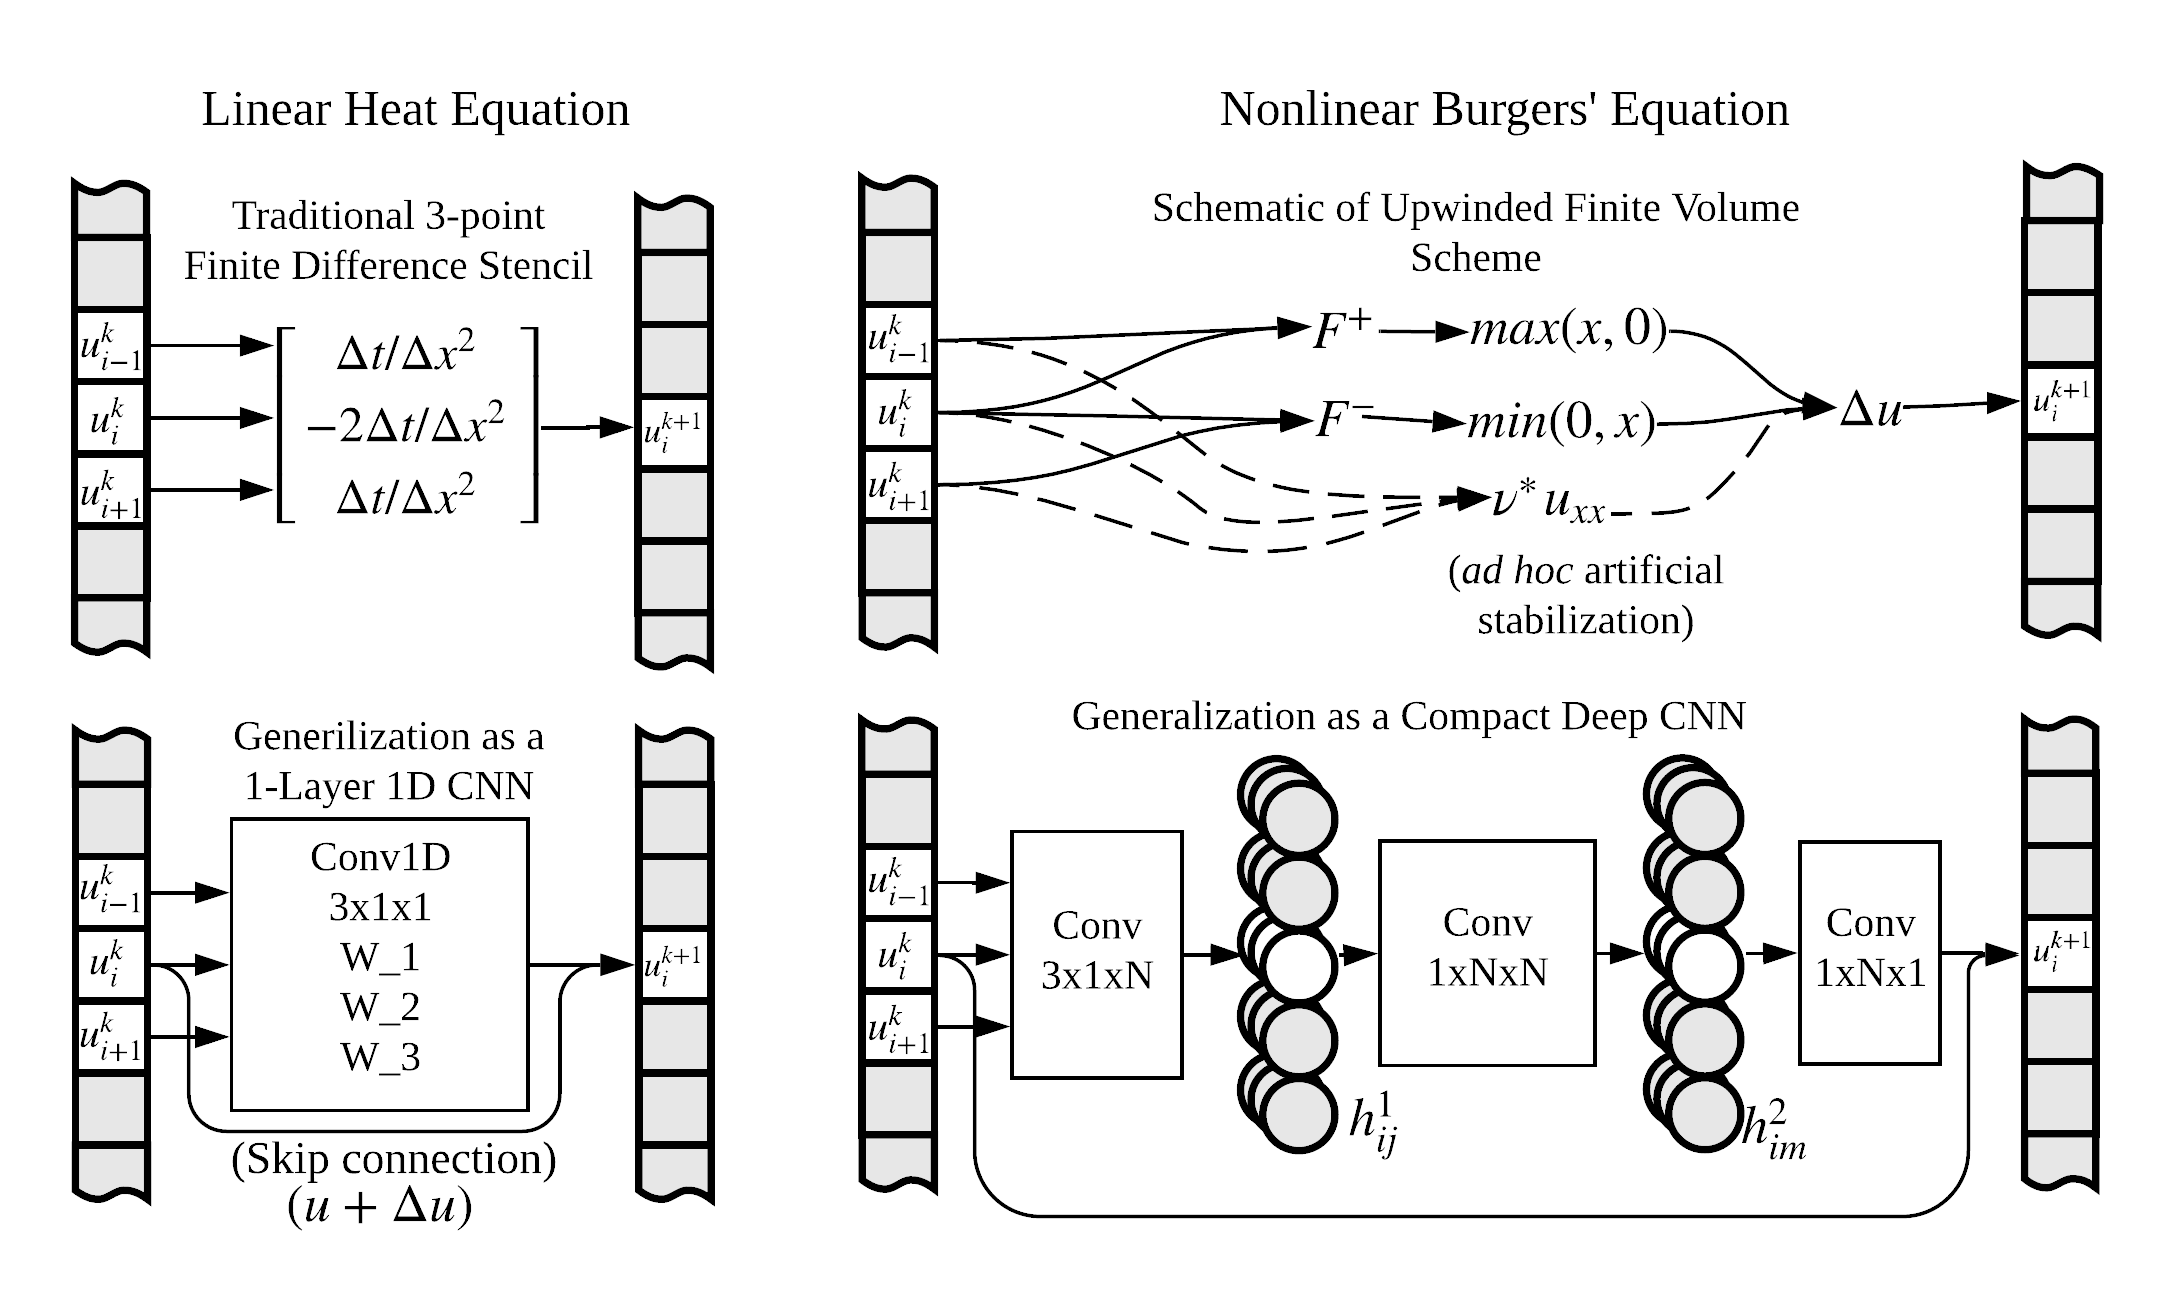
\includegraphics[width=5in]{CNN_FDM.png}  
  \caption{\label{fig:cnn_fdm}Coincidence of CNNs with existing finite difference
    schemes. On the left, a one-layer CNN is the same as the traditional 3-point finite difference
    stencil. It is demonstrated that the 3 weights converge to the
    expected parameters. On the left, a finite volume scheme for
    Burgers' equation requires a complex nonlinear graph with
    decision trees for winding and sometimes nonphysical stabilization terms. A generalized CNN can attempt to
    discover a similar, or even better, method. Including the skip connection
    allows the model to be generalized to other timestep sizes, and
    might improve recurrent training.}
\end{figure}

As illustrated in Figure \ref{fig:cnn_fdm}, some numerical schemes
can viewed as a fringe case of certain CNN architecture. The finite
difference method uses Taylor expansions to derive update rules for the next time step:
\begin{equation}
  u^{k+1}_{i} = u^k_{i}+\mathtt{stencil}\left( u^k_{i-1}, u^k_{i},u^{k}_{i+1}; \Delta x, \Delta t\right)
\end{equation}
The classical stencil for the heat equation is
$u^{k+1}\approx u^k+(k\Delta t)/(\Delta x^2) \left(u_{i-1} - 2 u_{i} +
  u_{i+1}\right)$.
This architecture corresponds to a fringe case ANN: a
3-weight 1D convolutional neural network (CNN) with no bias and no
activation function. Verifying that
these coefficients can be derived
by the learning strategy and optimization algorithm is proposed as a good first step.

% Compact means that only the first layer has width. Every successive
% layer is one-wide, and no pooling appears. This allows the network to
% be applied to a domain of any size, and enforces the locality
% constraint of the physics. Boundary conditions are enforced from the
% analytical solution when recurring in validation.

Forecasting far into the future is of interest. As a standard approach
in numerical methods, it is desired for a model to be able to recur on
its own outputs without lossing accuracy or stability:
$u^{k+n}=f(f(...f(u^k)$. The connection between numerical integration
and recurrence is in active study, with analogies to ANNs made by
\citet{chen_neural_2018} and \citet{chang_multi-level_2017}.
%The
%models learned in this study are judged based on ability to recur on
%validation initial conditions.

The 1D problems were specifically chosen to yield quickly reproducible
experiments. For each equation, a dataset
including different trajectories from different initial conditions is made
using analytical solutions with Sympy. These are evaluated on a grid of 41 points in $x$ and 100
snapshots in $t$, for a total size of $\approx$1.6MB. Each experiment runs
in a few minutes using a GPU. The
entire study is implemented in PyTorch. The source code, datasets,
and figures for this study can be found at https://github.com/{\em omitted for blind review.}


% Question: Do we want to learn $u^{k+1}$ or $\Delta u^{k+1}$?
% The paper THAT ONE ABOUT RESNET showed a technique to describe
% residual networks as iterative time stepping methods to improve
% training.
% The effect on training is tried by adding a skip connection to all of the models--- $f(x)=\mathbf{net}(x)+x$---so that $\mathbf{net}$ learns the rate. This would further allow changing $\Delta t$ or generalize to other time integration schemes, but this was not explored.


% performing recurrent prediction, the values at the edges of the domain are set to
% the known analytical solution to ensure that improper treatment of the
% boundaries do not contaminate the results, yielding pure Dirrichlet
% boundary conditions every. The boundary domain is extended to the
% sencil width. The model output is thus padded by the correct amount of 0s to make the output an $N_x$ array.


% \begin{table}
%   \caption{\label{tab:network}Network Architectures Used}
%   \begin{tabular}{llc}
%     \toprule
%     Name & Description & No. of Parameters \\
%     \midrule
%     PureStencil & Conv(1,1,3,bias=False) & 3 \\
%     PureLinear & Linear($N_x$,$N_x-2$,bias=False) & 1,599 \\
%     FCMLP & & \\
%     Linear Conv & & 3 \\
%     Pure-ConvMLP & &  \\
%     Autoencoder & & \\
%     U-Net & &  \\
%     Recurrent & & \\
%     \midrule
%     Discriminator & Conv(3,1),Pool(3,1), AdptPool(1), Sigmoid & \\
%     \bottomrule
%   \end{tabular}
% \end{table}




\section{The Heat Equation}

The first step to test the methodology is to derive the $[1,-2,1]$
stencil from a dataset of heat equation trajectories with a three-parameter CNN.
The dataset contains ten trajectories for various trigonometric and polynomial
initial conditions with $u=0$ boundary conditions computed with the
Fourrier series analytical solution. Two trajectories each are used for
testing and validation.
To ensure stability for an explicit scheme, the domain was $x\in[0,1]$,
$t\in[0,1/4]$ and the diffusion coefficient was
$k=1/10$, informed by the Courant–Friedrichs–Lewy (CFL) condition $\delta t\leq k \delta
x^2$\citep{leveque_finite_2007}.\footnote{As with implicit numerical methods, a
  different ANN architecture may be able to surpass this condition.}

% The standard metric is the L2 loss function:
% \begin{equation}
% L\left(u^k,u^{k+1}\right) = \left\| u^{k+1}_i-f(u^k) \right\|_2^2.
% \end{equation}

% % Multiple input steps effects the network architecture:
% \begin{equation}
% L\left(\left\{u^k,u^{k-1}...u^{k-P}\right\},u^{k+1}\right) = \left| u^{k+1}_i-f(u^k,...u^{k-P}) \right|
% \end{equation}

A combination of standard training using the mean squared error (MSE) and
adversarial training with a discriminator is considered. A conditional
discriminator $D(y|x)$ is optimized which learns, given $x$, to determine
if $y$ is the datum or the model prediction. For these problems, no
stochastic effects are included, and the model and evaluation of the
discriminator are deterministic. Thus, the
discriminator essentially {\em learns a loss function}, replacing the
mean-squared-error loss with potentially something better:
\begin{equation}
L\left(u^k,u^{k+1}\right) = \lambda_1 \left\| u^{k+1}-f(u^k)
\right\|_2^2 + \lambda_2\left(1 - D\left(f(u^k)|u^k\right) + D\left(u^{k+1}|u^k\right)\right)/2
\end{equation}
The cost function is the mean of the loss function over the batch.
%\footnote{Averaging this
  % loss function over a batch the same way as the others yields the
  % $\mathbb{E}_x[1-D(f(x))]-\mathbb{E}_y[D(y)]$ equation of
%traditional
  % GANs, but using ``expected value'' does not quite apply to a fully
  % deterministic model.}
The weights $\lambda_1$ and $\lambda_2$ are set to $(1,0)$, $(0,1)$, and $(1,1)$. When $\lambda_2\neq 1$, the
discriminator $D$ is trained to maximize the cost function alternating
steps with the model $f$.

% \begin{figure}
%   \centering
%   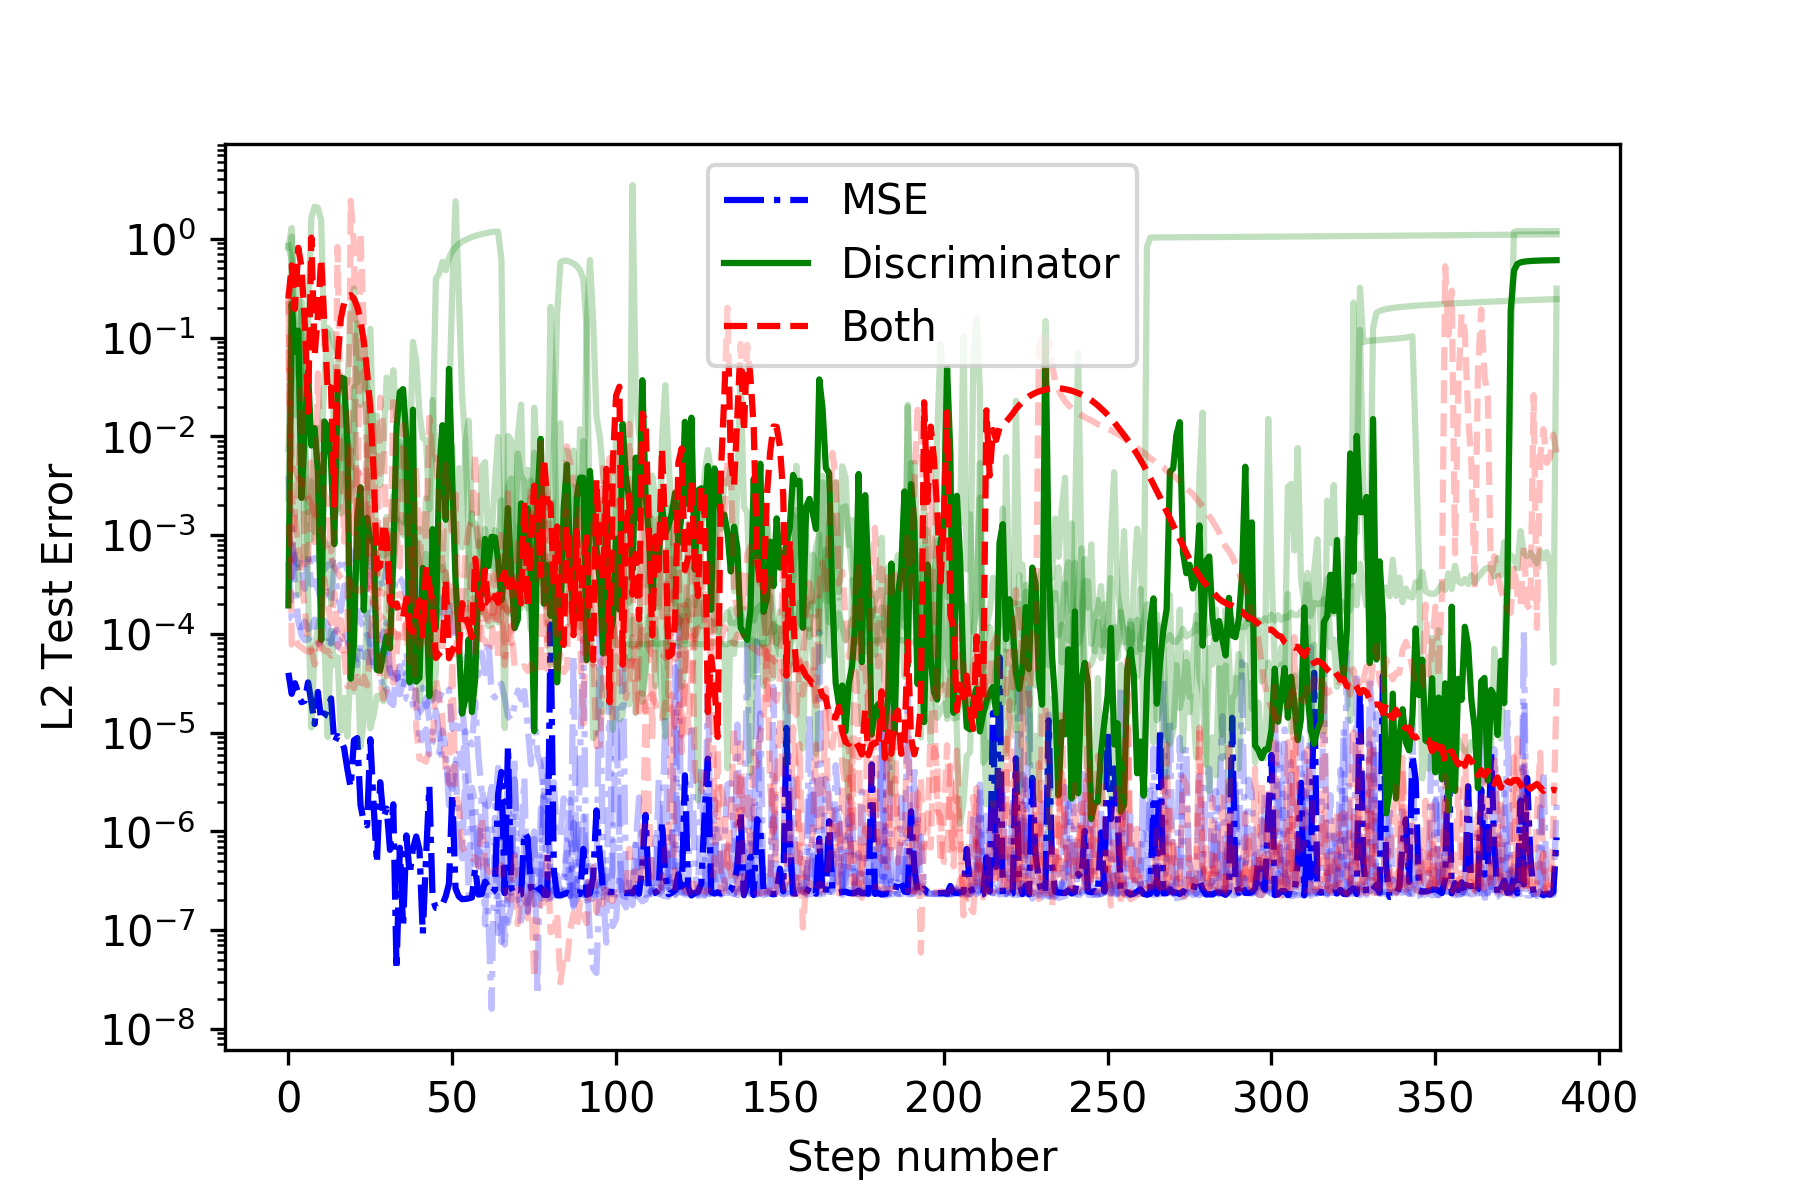
\includegraphics[width=5in]{3pt_L2_loss.png}
%   \caption{Convergence of 3-parameter CNN to the expected stencil
%     using L2 optimization and adversarial
%     training. $10^{-7}$ error is likely the best obtainable in single precision.}
% \end{figure}

\begin{table}
  \caption{\label{tab:conv}The convolutional weights learned for the
    heat equation for five randomly initialized runs with three
    training strategies. The weights are
    divided by $k \Delta t / \Delta x^2$ to normalize to
    $1,-2,1$. Training through a discriminator does not get the
    correct magnitude, but, interestingly, learns the shape.}
  \centering
  \begin{tabular}{rrr|rrr|rrr}
    \hline
    \multicolumn{3}{c}{MSE} & \multicolumn{3}{c}{Discriminator Adversary}  &\multicolumn{3}{c}{Both} \\
\hline
 0.997 & -1.995 & 0.997 & 1.398 & -1.149 & 1.401 & 1.073 & -2.149 & 1.077 \\
 0.997 & -1.995 & 0.998 & 1.058 & -3.196 & 0.956 & 0.994 & -2.000 & 0.995 \\
 0.998 & -1.996 & 0.998 & 1.512 & -0.824 & 1.624 & 0.595 & -1.502 & 0.732 \\
 0.998 & -1.994 & 0.999 & 1.084 & -1.154 & 1.116 & 1.000 & -2.001 & 1.000 \\
 0.998 & -1.995 & 0.998 & 1.392 & -0.558 & 1.394 & 1.000 & -1.999 & 1.000 \\
\hline
\end{tabular}
\end{table}


% Testing the algorithms ADAM, Rprop, and SGD on learning rates of
% $0.1,10^{-2}, 10^{-3}, 10^{-4}$, and $10^{-5}$,
%  only ADAM converged to the
% right answer with $0.1$ and $10^{-2}$. 
% Single precision with a learning rate of $0.1$ was used for the rest of the studies.

%This test also verified that the dataset met the CFL condition by
%assigning the CNN parameters to the expected answer.

The experiment was repeated 5
times for each loss function and the weights are reported in
Table \ref{tab:conv}.
The MSE loss achieves $10^{-7}$ error, which is likely the best obtainable in single precision.
Purely adversarial training with a discriminator continued for ten
times as many epochs and does not
learn the same stencil. It appears that the discriminator only learns
the shape, but not the magnitude. Combining the
discriminator loss and L2 loss did not succeed every time and
converged slower (in number of steps). 
%When observing the learned values during training, it was observed that the $[1,-2,1]$ ``shape'' of the stencil was trained quickly, but that it took a longer time to optimize to the magnitude.
The architecture of the discriminator was a pooling CNN with three
hidden layers and LeakyReLU activation functions, with a total of 51
parameters. Its architecture should be more thoroughly
studied to make a firm conclusion. Increasing from single
precision to double precision did not change the results.

\section{Burgers' Equation}

The dataset contained 20 trajectories with a series of linear profiles, shock and rarifaction
profiles of the Riemann problem, and one parabolic
profile. Anti-reflections were included to encode the symmetry.
%(These were the only analytical solutions of which the {\em author(s)}
are aware.)
The CFL equation for this equation is $\Delta t < C \Delta
x / \max lu|$, so the domain was set to $x\in[-1,1]$, $t\in[0,1]$, and
the velocities were kept below 2.


The compact deep CNN architecture has the following three hyperparameters: the number of
features in the hidden layers $n$,the total depth of the network $d$,
and the activation function, $\sigma$. The layering of the
architecture is: 
Conv(1,$n$,3), $\sigma$,Conv($n$,$n$,1)... $d-1$ times... $\sigma$,
Conv($n$,1,1).
The following activation functions were tried: ReLU, LeakyReLU, Tanh,
CELU, Sigmoid. The depth was varied from 2-4, and number of channels
from the set 3,5,10, and 15.
The width of the first convolution, 3, was not varied in this study,
but is under active research.

\begin{figure}
  \centering
  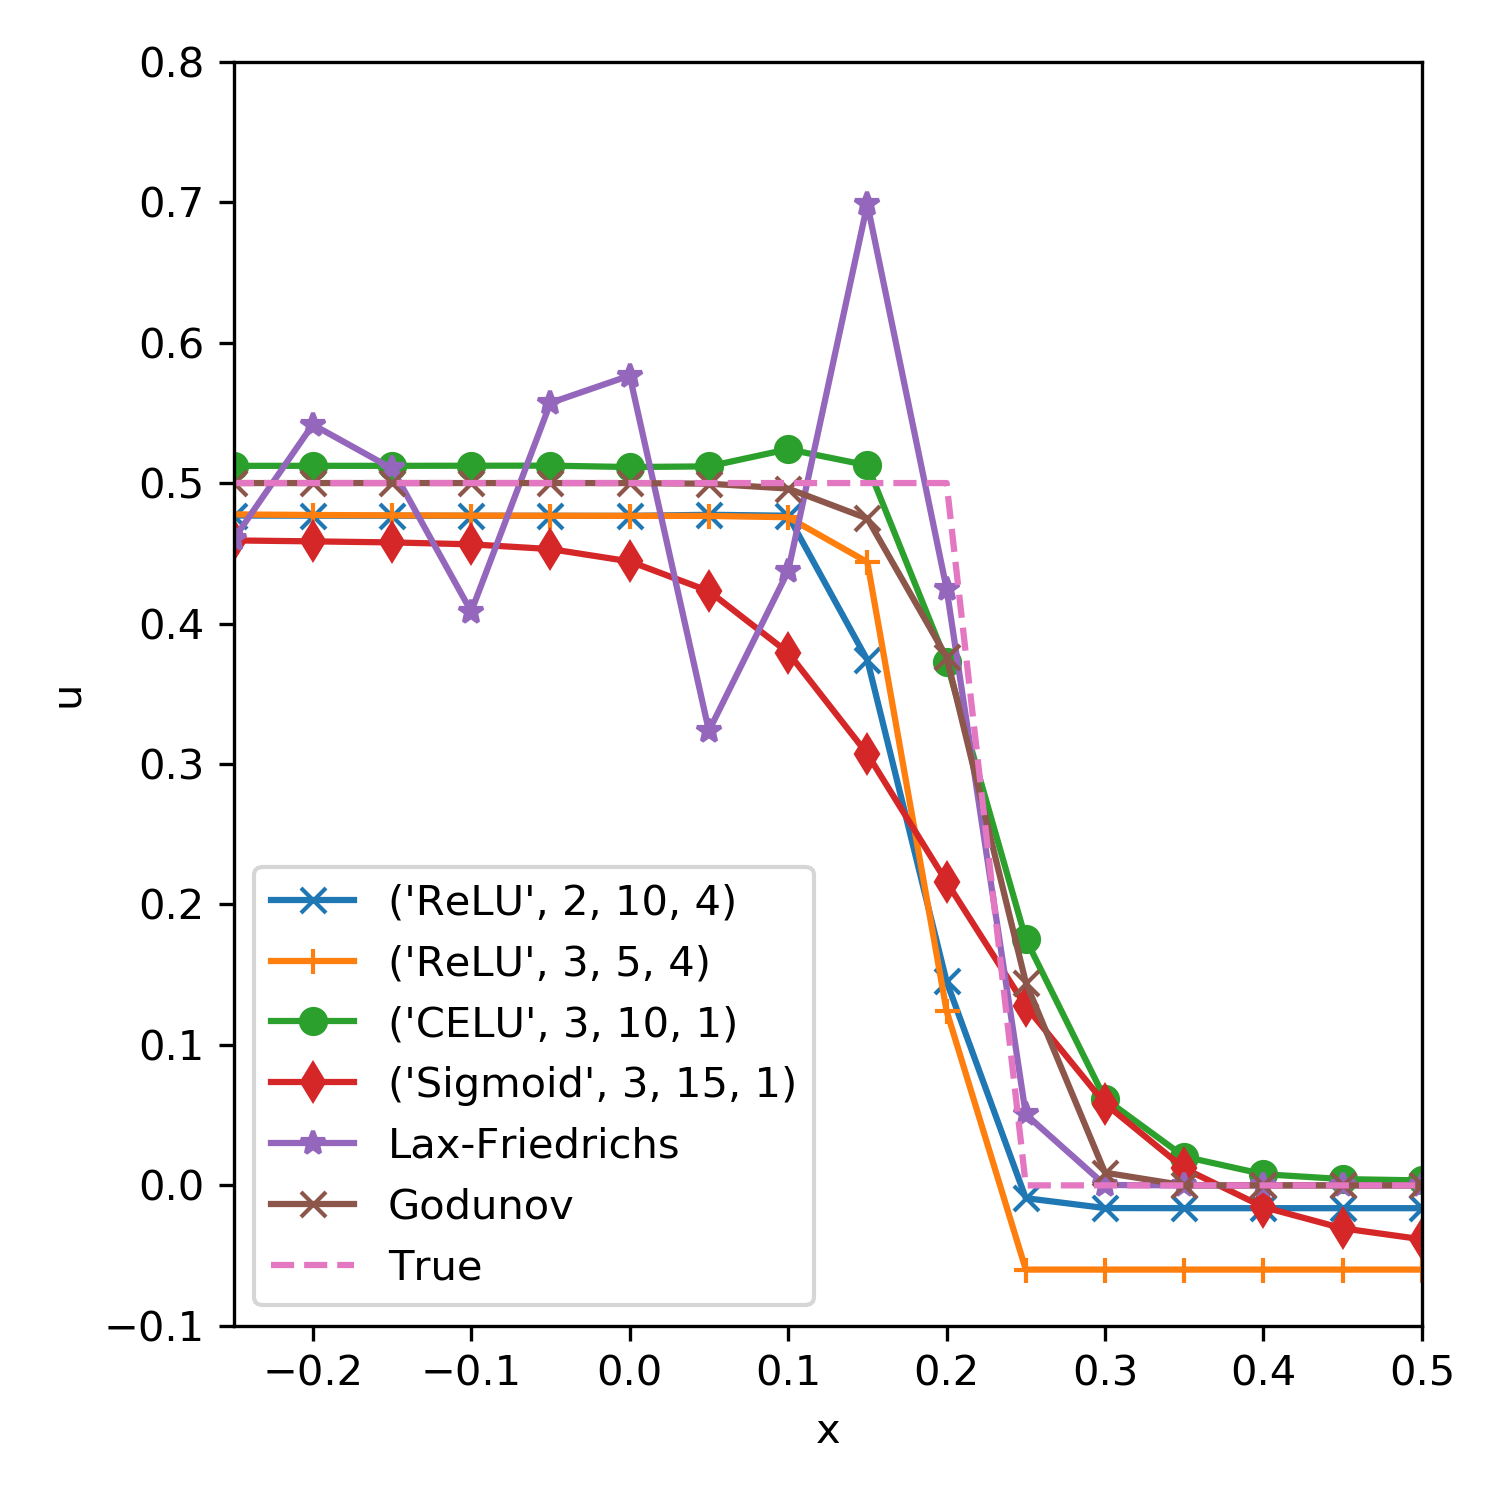
\includegraphics[width=2.75in]{shockwave_profile.png}%
  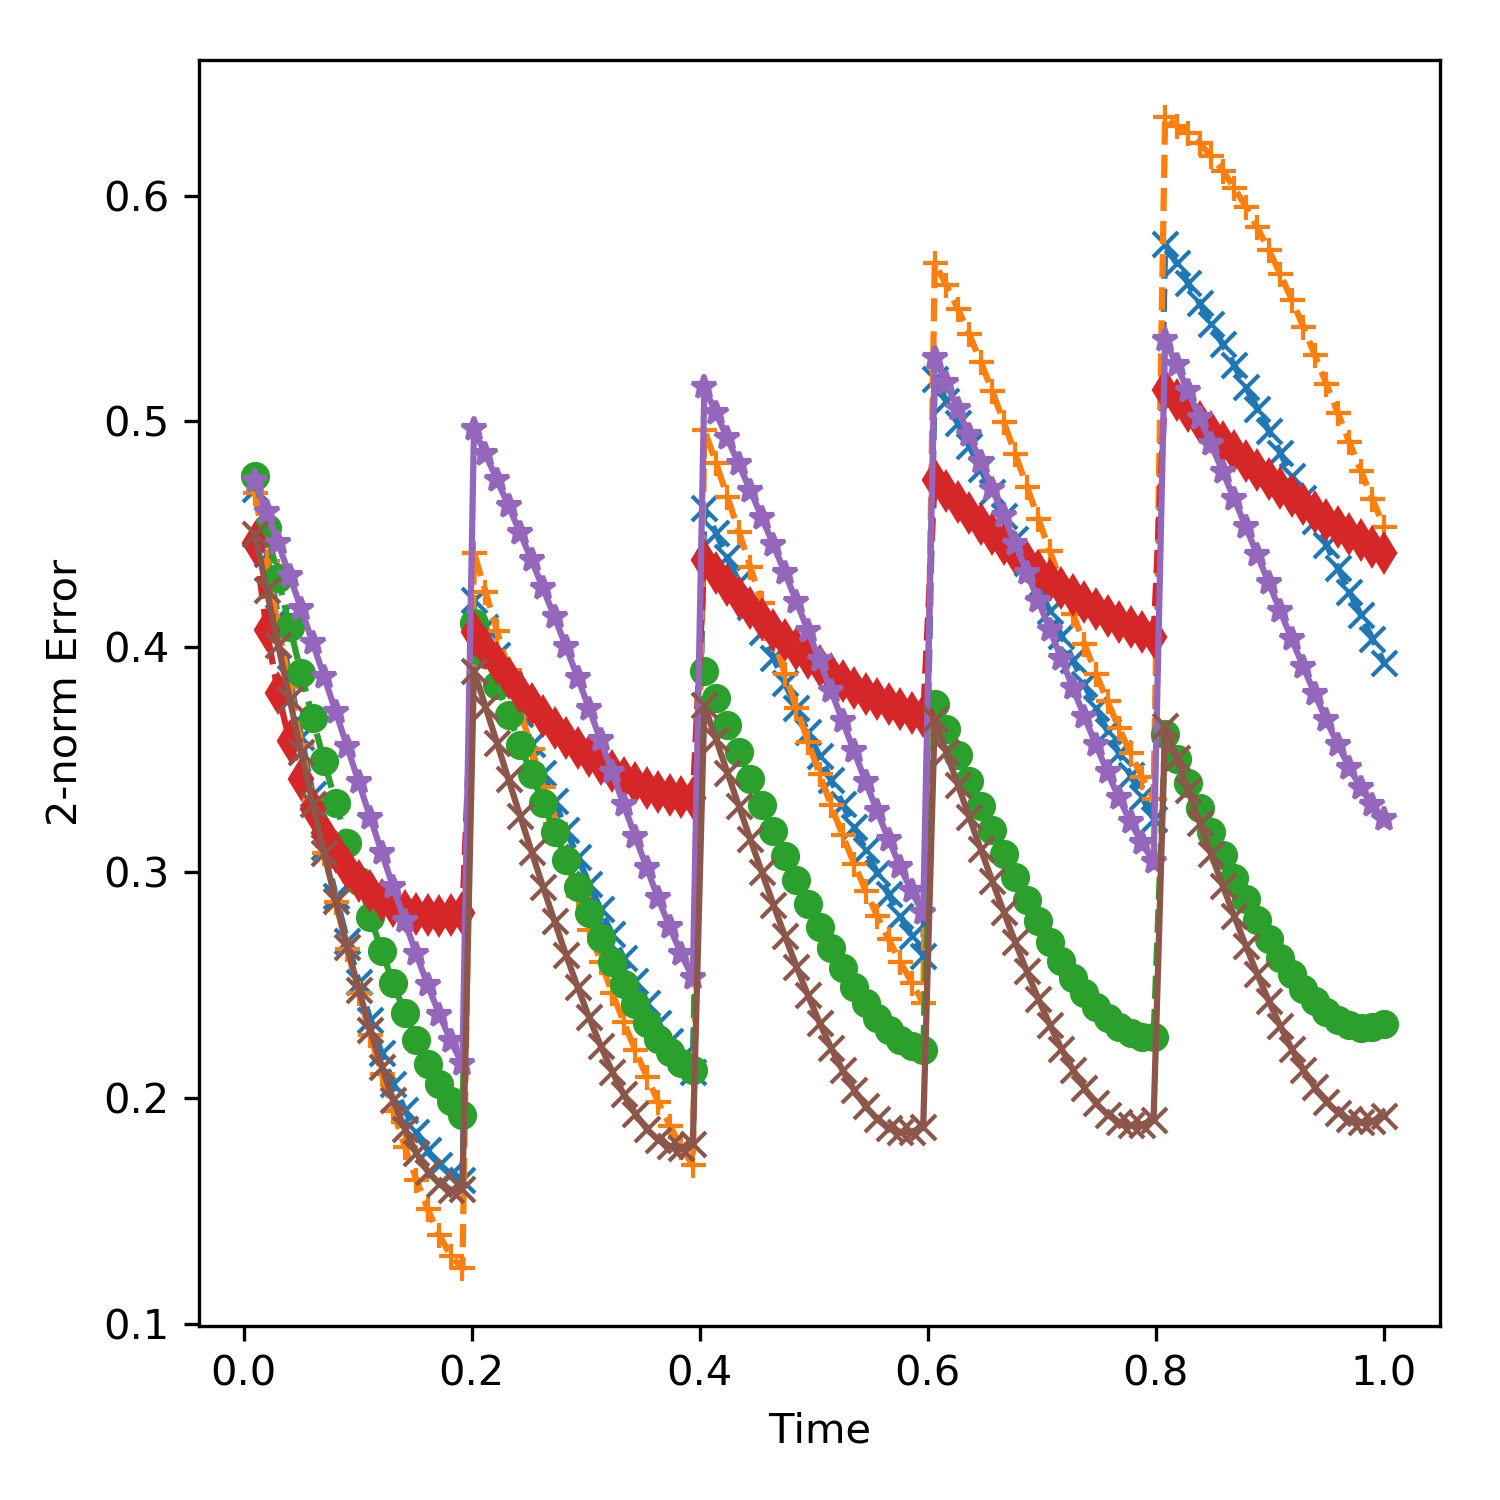
\includegraphics[width=2.75in]{shockwave_error.png}
  \caption{\label{fig:shock_comparison}Performance of the best learned models against well
    developed methods on a shock that did not appear in the
    training set. The legends are labeled by (activation, depth,
    channels, and terms in Eq. 4). Left, a snapshot of the methods with the true
    solution after 100 steps to $t=1$. (To stress: the CNNs recurred on
    themselves 100 times.) Right, error of the
    methods compared to the analytical solution over time. }
\end{figure}

To improve training with recurrent prediction as a goal,
multiple steps were included in the training:
\begin{eqnarray}
L\left(u^k,\left\{u^{k+1},u^{k+2},u^{k+3}...\right\}\right) =  \left\|
  u^{k+1}-f(u^k) \right\| + \lambda_1  \left\| u^{k+2}-f \circ f(u^k)
  \right\| ...\nonumber
  \\
   + \lambda_2  \left\| u^{k+3}-f \circ f \circ f(u^k) \right\| + ...
\end{eqnarray}
where $\lambda_i$ are weighting coefficients that were set to one in
this case. Hyperparameter variation using 1,2,3, and 4 steps
qualitatively demonstrated an
improvement in overall stability of the models. The search space included 180 different networks and loss
function combinations. Learning a discriminator did not have a positive effect on the
results for this problem.


The learned model is compared to implementations of the classical
numerical schemes of Lax-Friedrichs and Godunov. (See
\citet{leveque_finite_2007} and  \citet{godunov_difference_1959}.) This
profile did not appear in either training or testing. The final
profile and error across is shown in Figure
\ref{fig:shock_comparison}. 
The best learned model is less accurate than Godunov's, but performs
similarly. The Lax-Friedrichs method exhibits instability, a well
known-phenomenon. This behavior was seen in other model
architectures on other problems not shown. Further demonstrations with more model
architectures can be found online.

\section{Conclusion}
\label{sec:conclusion}

We show that a fringe case of CNN architecture corresponds to a
standard finite difference stencil, and converges to the expected
coefficients using popular optimizers for ANNs on the L2 loss but not with a
learned loss function through adversarial training.
These results suggest caution when using a purely GAN-type training for physics problems where accuracy is important. The ability to detect the shape of the operator is promising; the {\em author(s)} hypothesize that the discriminator may help with issues such as stability in more complex systems.
Deep CNNs were successfully learned for solving Burgers' equation accurately and stably.
By searching for compact models on small solutions, the model can be applied to domains
with different geometries.
%For Burgers' equation, a richer dataset with more variety would be beneficial.
% In Figure X, the model is applied to a domain with 2000 gridpoints
% on a function unlike anything in training.


% pecially designed models that enforce conserved quantities such as
% mass and energy, such as the work of \citet{bar-sinai_data-driven_2018} are
% advantageous, but this requires knowing the quantities {\em a
%   priori}. Future work seek to design conservative networks that can learn features
% that are conserved quantities.


Applying intuition from well understood physics-and-math-up approaches
will improve future approaches, providing insights that can hopefully
be applied to problems without known physical descriptions but
similarities to canonical problems. Studying the stability properties of recurring these networks applied
to physics problems can extend to stabilizing recurrent networks for
other applications.
By finding this area of overlap between solving PDEs and deep
learning, we can seek to bridge the gap and transfer knowledge between
the two fields.

% paper checks the methodology on this sim

% This analogy allows us to interpret the output of our learning algorithms, and guide the design of new architectures for these problems.
% This work hopes to provide a simple, well understood benchmark for
% testing recently demonstrated ML methods for solving physical systems
% developing ML methods for solving physical systems.
% Next steps will look for which NN architectures can perform
% forecasting at time steps beyond the CFL condition.

%For example, can methods for higher orderfor L-stable implicit high-order ODE integration be applied to transformer networks?

% \subsection{Margins in \LaTeX{}}

% Most of the margin problems come from figures positioned by hand using
% \verb+\special+ or other commands. We suggest using the command
% \verb+\includegraphics+ from the \verb+graphicx+ package. Always specify the
% figure width as a multiple of the line width as in the example below:
% \begin{verbatim}
%    \usepackage[pdftex]{graphicx} ...
%    \includegraphics[width=0.8\linewidth]{myfile.pdf}
% \end{verbatim}
% See Section 4.4 in the graphics bundle documentation
% (\url{http://mirrors.ctan.org/macros/latex/required/graphics/grfguide.pdf})

% A number of width problems arise when \LaTeX{} cannot properly hyphenate a
% line. Please give LaTeX hyphenation hints using the \verb+\-+ command when
% necessary.

\subsubsection*{Acknowledgments}

{\em Placeholder for blind review.}
% Use unnumbered third level headings for the acknowledgments. All acknowledgments
% go at the end of the paper. Do not include acknowledgments in the anonymized
% submission, only in the final paper.

% \section*{References}

% \medskip

% \small

\bibliographystyle{plainnat}
\bibliography{zotero}

\end{document}